\section{City Generation Architecture}
\label{sec:city-gen-arch}

In order to approach the problem of 3D city generation it was necessary to first break it down into manageable modules that could be worked on in parallel.
One of these modules had to be responsible for the GUI presented in the previous subchapter.
This module was named \textit{Application} and could be kept relatively small as most logic would be handled by the Unity engine.
There also needed to exist some module responsible for the PCG, since that is the core of this research.
This module was named the \textit{WorldGenerator}.
\textit{WorldGenerator} was then further split into eight submodules that would each be responsible for a distinct part of the model generation.

The implementation of the user interface would be rather simple and was thus treated as a single module, while the generation needed some architecture to handle the communication between submodules.
The two main architectures considered for the generation were a function-based and a pipeline-based approach (see Figure~\ref{fig:architecture_approaches}).

The pipeline had the advantage of less overhead since each generator would directly (or through an interface) pass data onto the next.
However, this lack of overhead could impose limitations and there still needed to exist some module responsible for receiving and exporting all the generated model data.
Furthermore, when Blomqvist et al. developed a PCG engine, they experienced issues with their pipeline architecture, such as interconnected modules and bias of workload towards the early pipeline stages \cite[p. 45]{ba_landscape}.
Thus, with these concerns in mind, it seemed reasonable to settle for the function-based architecture instead.

\begin{figure}[h!]
  \centering
  \begin{subfigure}[b]{0.48\textwidth}
    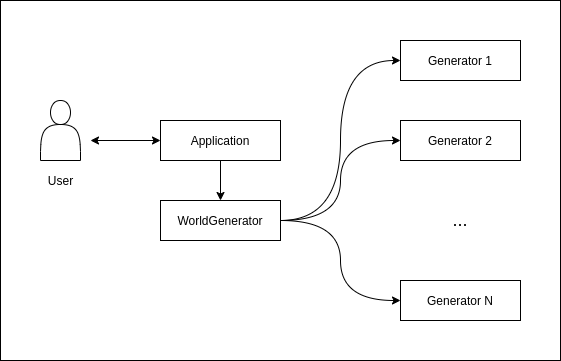
\includegraphics[width=\textwidth]{figure/architecture_functions.png}
    \caption{Function-based architecture. Each sub-generator is treated as an isolated function and \textit{WorldGenerator} controls how and when they are invoked.}
  \end{subfigure}
  \quad
  \begin{subfigure}[b]{0.48\textwidth}
    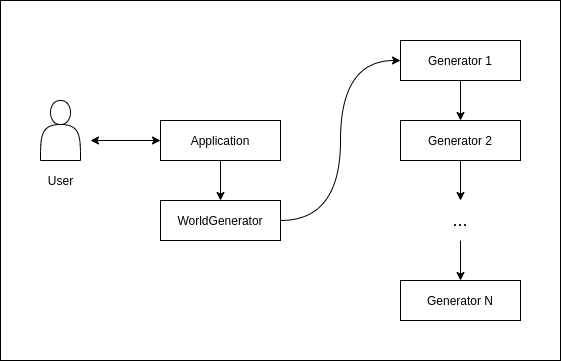
\includegraphics[width=\textwidth]{figure/architecture_pipeline.png}
    \caption{Pipeline-based architecture. The first generator is invoked by \textit{WorldGenerator}, and then each sub-generator passes on its output to the next sub-generator.}
  \end{subfigure}

  \caption{Two different architecture approaches considered for the generation logic.}
  \label{fig:architecture_approaches}
\end{figure}

The function-based architecture showed several promising advantages.
For one, each generator would only receive input that it actually depended on, while with a pipeline each generator would have had to pass along all its data.
This separation not only makes debugging easier, but it also improves performance slightly.
Another recognized advantage was that generators could now be run asynchronously and in separate threads, further benefiting performance.
Lastly, as generation steps would be invoked from GUI buttons, possibly in non-linear order and with \textit{undo} operations, it was better suited if \textit{WorldGenerator} could communicate with each sub-generator directly.
Consequently, the function-based architecture was chosen.

\begin{table}[H]
  \centering
  \begin{tabular}{lllll}
    \textbf{Input}                           &               & \textbf{Function}            &               & \textbf{Output}         \\
    \midrule
    \textit{Size, Offset, SeaLevel}          & $\rightarrow$ & \textbf{TerrainGenerator}    & $\rightarrow$ & \textit{Terrain}        \\
    \textit{Terrain, PopulationAmplifier[]}  & $\rightarrow$ & \textbf{PopulationGenerator} & $\rightarrow$ & \textit{PopulationMap}  \\
    \textit{Terrain, PopulationMap}          & $\rightarrow$ & \textbf{RoadGenerator}       & $\rightarrow$ & \textit{RoadNetwork}    \\
    \textit{RoadNetwork, PopulationMap}      & $\rightarrow$ & \textbf{BlockGenerator}      & $\rightarrow$ & \textit{Block[]}        \\
    \textit{Block, PopulationMap}            & $\rightarrow$ & \textbf{PlotGenerator}       & $\rightarrow$ & \textit{Plot[]}         \\
    \textit{Plot, Terrain, Population}       & $\rightarrow$ & \textbf{BuildingGenerator}   & $\rightarrow$ & \textit{Building}       \\
    \textit{Plot, Terrain}                   & $\rightarrow$ & \textbf{ParkGenerator}       & $\rightarrow$ & \textit{Park}           \\
    \textit{Plot, Terrain}                   & $\rightarrow$ & \textbf{ParkingGenerator}    & $\rightarrow$ & \textit{ParkingLot}     \\
    \bottomrule
  \end{tabular}

  \caption[]{The proposed generator functions needed to generate the 3D cities. The invocation of these functions are handled by \textit{WorldGenerator}. '\textit{[]}' denotes plural (e.g. list or array) of the preceeding data structure.}
  \label{table:generators}
\end{table}
\vspace{-0.4cm} % Mimic spacing below figures

An overview of the eight generators that were decided upon is shown in Table \ref{table:generators}, while the implementations and responsibilities of these generators will be detailed in the following subchapters.

\subsection{Terrain Generation}

\begin{table}[H]
 \centering
 \begin{tabular}{lllll}
  \textbf{Input} & & \textbf{Function} & & \textbf{Output} \\
  \midrule
  \textit{Size, Offset, SeaLevel} & $\rightarrow$ & \textbf{TerrainGenerator} & $\rightarrow$ & \textit{Terrain} \\
  \bottomrule
 \end{tabular}

 \caption{Definition of the TerrainGenerator function which is responsible for generating the terrain.}
 \label{table:terrgen}
 \end{table}
\vspace{-0.4cm} % Mimic spacing below figures


The terrain generator constructs the landscape on which the city can be assembled.
It generates a mesh congregated out of triangles and a Perlin noise generator to apply height to the triangles' connection points.
Naturally, other generators need to take into account the height of the terrain and avoid uninhabitable areas like water and very steep hills.
The mesh is then textured by applying one texture to the terrain.
Colours of the texture blends between other colors depending on the height level of the terrain and water to illustrate the ground type at the current height level.

Cities could have been generated on a flat plane, which does have its advantages since more time could be spent on additional aesthetic details for the city.
However, a city surrounded by a landscape would result in a more realistic and vivid setting, which would indirectly make the city look better than if it were generated on a flat surface.
A plane that could simulate a basic, yet somewhat realistic, environment for the city to be generated upon was a self-evident feature that would be included in the project.
The generated environment would be decided to be referred to as terrain.
This terrain would be based on real-world aesthetics and therefore include natural biomes such as snowy mountains, grassland, hills and bodies of water, specifically oceans/lakes.
Additional aspects would bypass the range of the project's goals since the core focus of this project was the city, not the terrain.
Therefore, a decision was made to keep the terrain looking rather primitive, i.e. that it would be limited and expected to include: 

\begin{easylist}
 @ A mesh to represent the ground.
 @ The terrain's shape, as in bumps, hills, and valleys.
 @ A simple, flat plane clipping through the terrain to represent water.
 @ Colour and texture for water and ground depending on the height of a certain point on the terrain.
\end{easylist}

There were two ways the terrain base could have been created: either using a custom mesh made of triangles, or using an advanced, built-in terrain mesh API provided by Unity.
Both options had their advantages and disadvantages.

\begin{figure}[H]
  \centering
  % Use two minipages to add padding for the figure and its caption
  \begin{minipage}{.45\textwidth}
    \centering
    \begin{minipage}{.9\textwidth}
      \centering
      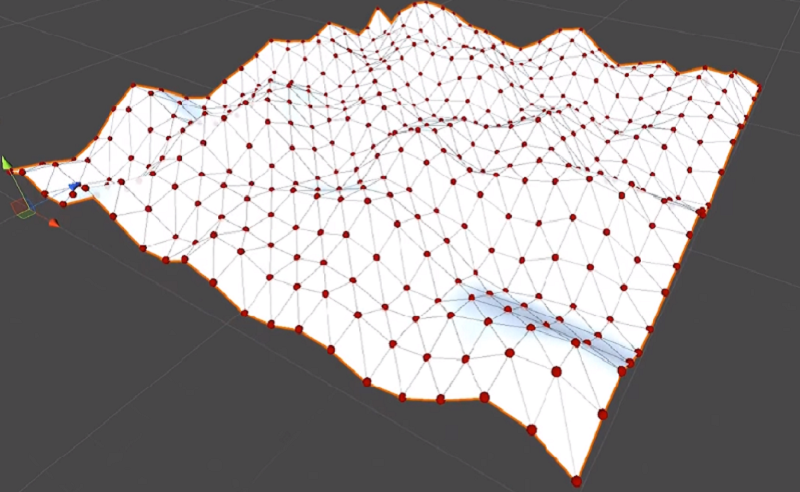
\includegraphics[width=\textwidth]{figure/terrain_mesh.png}
      \caption{Visualization of the mesh. The triangles in this picture are scaled up greatly.}
      \label{fig:terrmesh}
    \end{minipage}
  \end{minipage}
  \begin{minipage}{.45\textwidth}
    \begin{minipage}{.9\textwidth}
      \centering
      \centering
      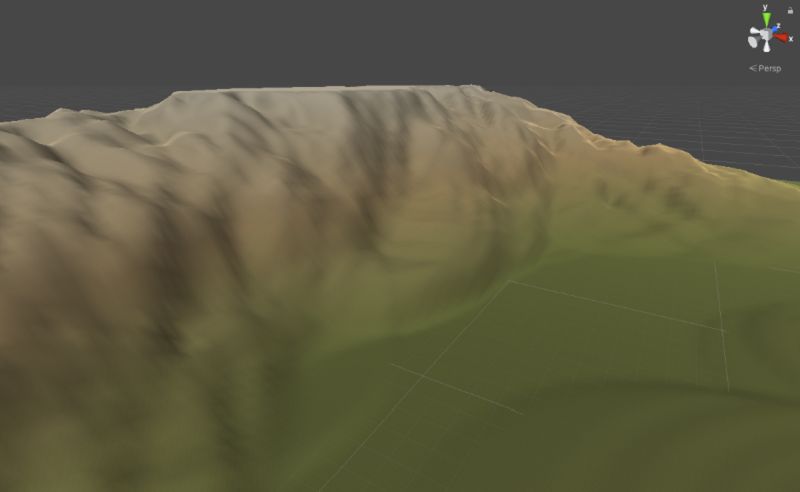
\includegraphics[width=\textwidth]{figure/terrain_API.png}
      \caption{Preview of a primitive terrain mesh using Unity Terrain API.}
      \label{fig:terrAPI}
    \end{minipage}
  \end{minipage}
\end{figure}

Meshes consists of triangles connected to one another, similar to \ref{fig:terrmesh}.
However, height-based texture splatting could be problematic using this alternative, for the reason that a custom shader would have to be coded that performs the blending of textures.
This would lead to issues when exporting the terrain, along with the fact that more programming has to be done for this task.
On the other hand, the API is easy to get started with, because of its extensive documentation to encompass its functionalities.
For instance, texture splatting is incorporated into the API, which would make the process of generating textures much simpler.

In the first iteration for the terrain base, the API by Unity seemed reasonable as a primary choice due to its simplicity and availability.
Unfortunately, the API did not produce traditional meshes, and instead produced dynamically adapting objects specific to Unity.
Converting the object could be done using Unity Editor packages; however, those tools would be inaccessible when compiling the final application, and including them in it did not seem possible.
Because of this, the terrain was refabricated with a custom mesh.
To counteract the need to program a custom shader, the terrain only contained one texture, which was gradually saturated with a different color to illustrate the expected type of ground existing on that height level.
Specifically, the texture's color would be shifted toward a white color to illustrate mountain tops, brown color for hills, green for low ground grassland, and a beige-yellow color for heights slightly above water.
Water is unaffected by this.

The next decision was to pick an algorithm that could designate height levels for the flat terrain, i.e. to shape it with inward and outward-facing dents that would represent valleys/ocean and mountains, respectively.
It was decided that the terrain was to be procedurally generated, as it would allow drastically more varied content in the generator.
The most common algorithms considered that could solve the procedurally generated landscape were simplex noise and Perlin noise.
If the height value from one of these functions were applied to the height value of each point, it would shape the terrain in a way similar to the real world.

Finally; appearance.
A blank, white canvas would not be appropriate as an environment, as it would appear glaringly unrealistic.
Therefore textures were implemented to grant the terrain the appearances of grass, mountains, water, etc. to showcase their existence, coloured as explained previously.
These following bullet points were the goals for the appearance of the terrain:

\begin{easylist}
 @ Oceans and lakes should have a blue tint.
 @ Terrain slanting towards oceans with low steepness should transition into beaches.
 @ Spacious plains should cover various shades of green.
 @ Mountains should appear rocky.
 @ Tall mountain peaks should be covered in snow.
\end{easylist}


\subsection{Population Generation}

The population generator will, as the name suggests, populate the terrain provided as input. Specifically, a heat map will be generated in the background of the terrain which will represent the population density for the entire plane.
The heat map is given by the noise module, and this invisible heat map can be brought forth within debug mode.
The areas of high density population can be altered with user input.
When generating the population map, the user will get a visual option to choose a location for a city, which is a point on the terrain of which the radius can also be customized.
On this marker, the population density of that area will be drastically increased.

The population generator was responsible for creating a procedurally generated intensity map describing the population in the world.
High intensity areas meant that there was a higher density of the population.
Multiple generators in the sequence required a population map to create more realistic buildings, thus the population map needed to reflect the landscape accordingly.
Because of that, the population map was responsible for the rough shape of the city.

To generate an intensity map, it required the terrain parameter, which was used to mask off certain areas in the landscape, such as oceans, rivers or mountains.
Then, the generator would use a few layers of simplex noise to create a representation of populations throughout the world.
Population markers were used to increase population density in a certain area, and these were applied after generating the initial population map.
This was useful for making sure the center of cities have a higher density, but it would still respect the original population map to some degree.
In figure 4.2, a population marker was placed in the center of the city, which meant the population density was much higher there.
White areas have a higher population density, dark areas have a lower population density. This figure also shows that main roads outside the cities will tend to shy away from lower-density areas, but not always.

\begin{figure}[h!]
  \centering

  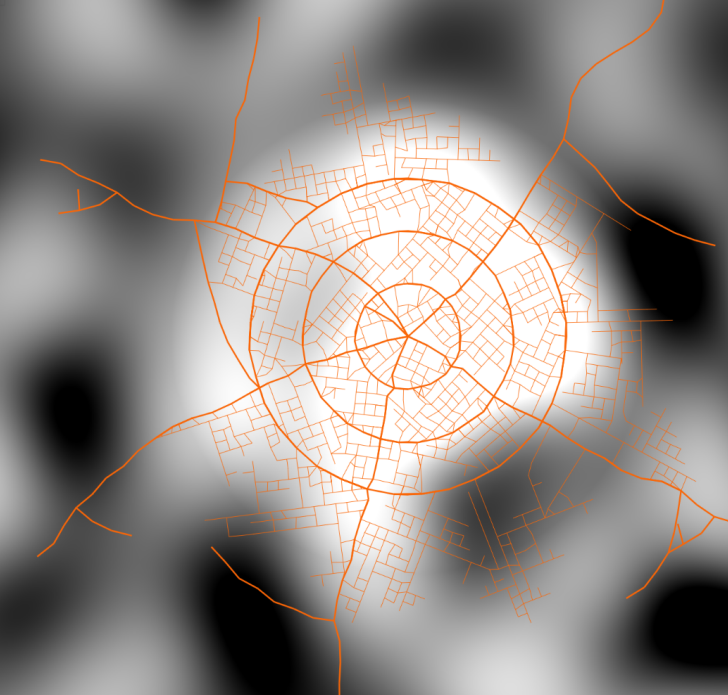
\includegraphics[width=0.8\textwidth]{figure/pop_density.png}
  \caption{An example of a population map with a Paris city generated within it.}

  \label{fig:population density}
\end{figure}
\subsection{Road Generation}

The fundamental infrastructure of a city is the road network and, as such, it was important that the road generation would be both flexible and offer realistic results.
To generate such networks, the RoadGenerator function was designed (see Table~\ref{table:def_roadgen}).

\begin{table}[H]
  \centering
  \begin{tabular}{lllll}
    \textbf{Input} & & \textbf{Function} & & \textbf{Output} \\
    \midrule
    \textit{Terrain, PopulationMap, Markers} & $\rightarrow$ & \textbf{RoadGenerator}       & $\rightarrow$ & \textit{RoadNetwork}    \\
    \bottomrule
  \end{tabular}

  \caption{Definition of the RoadGenerator which is responsible for generating road networks.}
  \label{table:def_roadgen}
\end{table}
\vspace{-0.4cm}

This function uses the terrain to place down roads, the population map to determine where roads are needed, and input markers to form city center patterns.

Three approaches were considered when designing the road generator.
The first was based on a recursive approach where the world was divided into cells with roads placed between the cells, forming a similar structure to Voronoi Diagrams.
However, this type of algorithm did not provide realistic-looking results.
Regardless of being flexible, it was overly complicated for the purpose of creating realistic road networks.
The second approach was search-based and would involve ML to produce structures based on data.
However, proper data appeared difficult to gather and evaluation of candidate solutions would become highly challenging.

The final approach that was decided to be used in the project involved an Agent-based generation which simulated road workers traversing the terrain.
The sole purpose of these Agents was to create roads based on different road building strategies.
Agents could also decide to branch into multiple new Agents, forming intersections in the road network.
Which strategy to use depends entirely on the goal of the generation, but the focus of this project has been to create a flexible base that could be extended to mimic any type of city generation.
As such, this project only includes Paris and Manhattan strategies, with the generation of main roads depending on the city strategy in order to achieve the aesthetics of the specific city type.
Paris-like cities have distinct rings within the city boundaries, while Manhattan-like cities follow a much more grid-like structure.

Furthermore, strategies may instruct the Agent to switch strategy mid-generation, be it randomly, or depending on some variables that the strategy has access to.
For example, if a strategy detected a relatively low population density, it might instruct the Agent to switch to a village-type strategy that could produce smaller villages with a different layout than cities like Paris or Manhattan.

Strategies can also define the configuration of the Agent, such as step size, how many steps an Agent can take before terminating (step count), and how many times an Agent can branch.
The strategy that the Agent uses is responsible for deciding when an Agent should terminate, except for step count which is handled automatically for all strategies.

The road generator uses the city markers as input to create the initial Agents that will start creating the road network.
Each city type needs its own preset arguments for the Agents, and this was solved by assigning an Agent factory to each city type.
The goal of the Agent factory is determining starting conditions for Agents depending on city type.

In Figure~\ref{fig:road_network_paris}, the road generator started by creating a ParisAgentFactory, which takes the city position and radius as input, and spawns multiple Agents depending on random variables within the bounds of the input.
The Agents are given a Paris-like strategy, which instructs the Agents to generate rings around the city center as well as main roads extending outwards.
This particular strategy was configured to have a very aggressive branching, which in turn produces lots of intersections.

A similar, but a more basic approach, was applied to the Manhattan strategy, but instead of rings, multiple straight main roads were generated (see Figure~\ref{fig:road_network_manhattan}).

\begin{figure}[H]
  \centering
  % Use two minipages to add padding for the figure and its caption
  \begin{minipage}[b][][b]{.3825\textwidth}
    \centering
    \begin{minipage}[b][][b]{.9\textwidth}
      \centering
      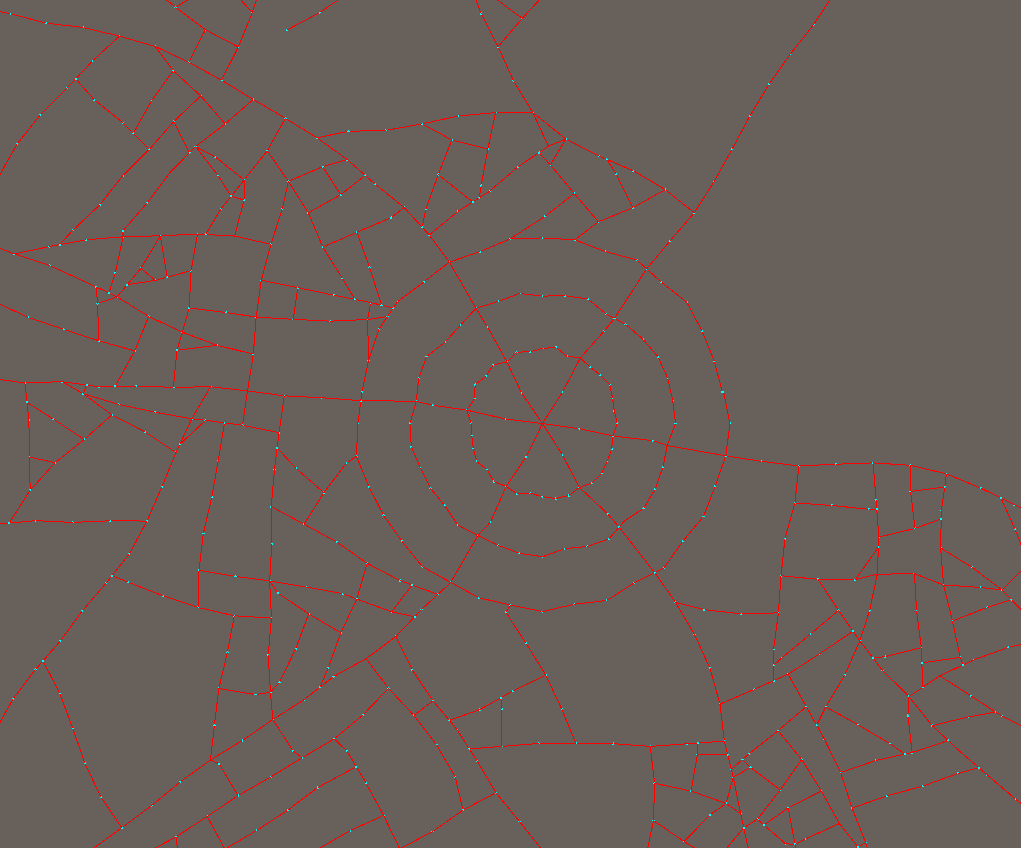
\includegraphics[width=\textwidth]{figure/road_network_paris.png}
      \caption{Example of the Paris road strategy.}
      \label{fig:road_network_paris}
    \end{minipage}
  \end{minipage}
  \begin{minipage}[b][][b]{.5175\textwidth}
    \begin{minipage}[b][][b]{.9\textwidth}
      \centering
      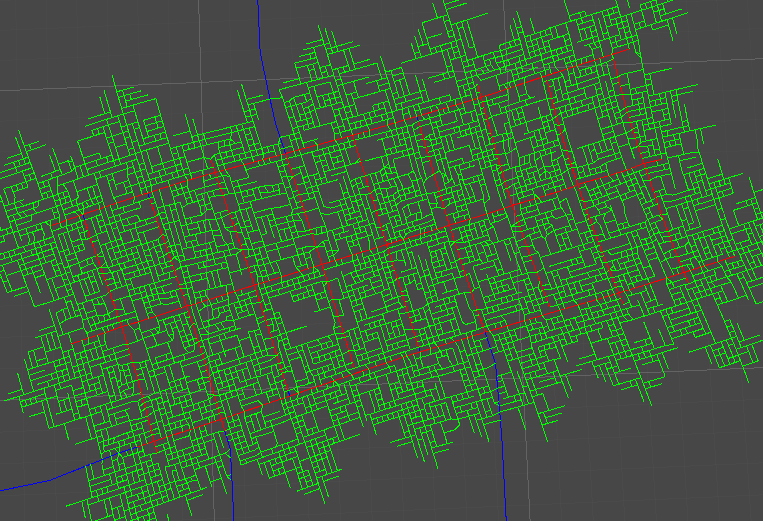
\includegraphics[width=\textwidth]{figure/road_network_manhattan.png}
      \caption{Example of the Manhattan road strategy.}
      \label{fig:road_network_manhattan}
    \end{minipage}
  \end{minipage}
\end{figure}


%% Intersection logic %%

While strategies handle how the Agent move, they do not decide how the roads should be placed.
When an Agent decides to place a road, it will attempt to find nodes in the nearby area to snap to.
If no such nodes are found, it will create a road between its previous position and its new position, and any roads that exist on the path in-between will be combined into an intersection.
Figure~\ref{fig:road_connection_cases} demonstrates the intersection created after an Agent attempts to cross another road, as well as an optimization technique making use of an R-Tree data structure \cite{wiki:R-tree}.

The R-Tree is necessary to quickly search for intersecting roads by avoiding to iterate over all nodes in the road network, or else the performance would result in an unusable application.
Each node is placed in the R-Tree with a bounding box that encapsulates each connecting node.
When two nodes are connected, the road network will search for nearby nodes that intersect with the bounding box of the new connection, as well as a snap radius.

There are a few cases where it is preferable not to create new nodes for Agents, but rather snap to nearby nodes or network edges.
The algorithm tests for four different cases, visualized in Figure~\ref{fig:road_connection_cases}.

\begin{figure}[H]
  \centering

  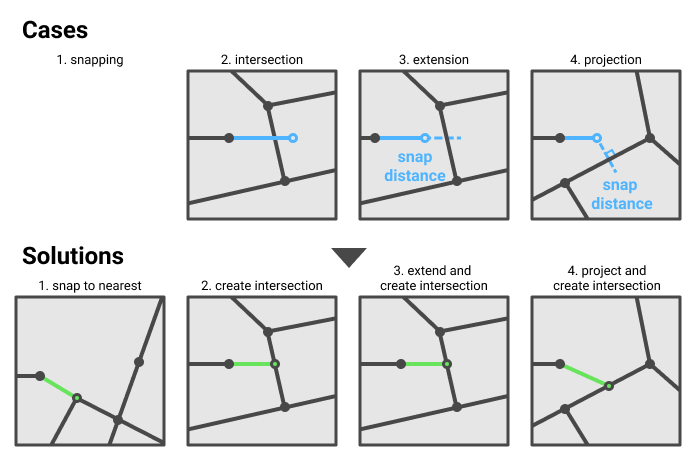
\includegraphics[width=0.8\textwidth]{figure/road_connection_cases.png}
  \caption{Four different cases that are handled in the road network connection logic.}

  \label{fig:road_connection_cases}
\end{figure}

% Move below? The caseenum should probably directly below the figure.
The solutions to the first three cases are similar to those found in the description of the snapping algorithm in the CityGen paper \cite[p. 6]{citygen_paper}, but these were not enough as it often happened that nodes still appeared close to roads without creating an intersection.
To combat this, the solution in the fourth case was added.

\begin{CaseEnum}
  \item The algorithm searches for nodes along the path to the new node, as well as within a radius around the node.
  The distance it searches for is defined in the Agent configuration, which any strategy can define.
  If a node is found, a connection between the previous node and that node will be made, making sure to re-run the algorithm in case paths are blocking.

  \item When there is a road between the origin node and the destination node, a new node will be created, splitting the road where the intersection point is.
  The destination node is then discarded, and the connection will be made from the origin node to the new node that was created.
  Agents will always stop at the intersection point instead of where it attempted to place the destination node.

  \item There are cases where an Agent lands just slightly before another road, but not near enough any other nodes.
  In these cases, the best approach is attempting to extend the node forward a certain distance (the snapping distance), and check if any other roads are intersecting.
  If any are found, split the road at the intersection point and connect the origin node to the intersection node.

  \item The final case occurs when the angle of approach relative to another road is small enough that the extension in the previous case will fail because the intersection point is further away than the snapping distance.
  To solve this, the network checks if there are any roads nearby by creating a perpendicular projection onto onto those roads.
  If the distance to that projection point is within the snapping distance, the same solution is applied as in \textbf{Case 3}.
\end{CaseEnum}

First, the algorithm will search for nodes along the path to the new node, as well as a radius around the node.
The second test attempts to \textit{``extend''} the node further forward, and if it intersects with an edge, it will create an intersection there.
The last test does another intersection test, but instead of extending the node forward, it will project the node to nearby edges and create an intersection there if it is within the snap radius.


\begin{wrapfigure}[11]{r}{0.3\textwidth}
  \centering
  \raisebox{0pt}[\dimexpr\height-2\baselineskip\relax]{
    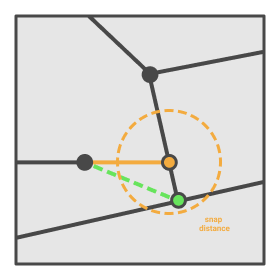
\includegraphics[width=0.26\textwidth]{figure/road_intersection_final_test.png}
  }
  \caption{Example of the test step before intersection node is created.}

  \label{fig:road_intersection_final_test}
\end{wrapfigure}

While these cases solve most of the issues in the road network and make sure Agents are not creating unnecessary roads, it is still not enough to guarantee a good-looking road network.
In cases 2, 3, and 4, one question that came up was \textit{``what happens if the node that was created at the intersection is too close to one of the nodes at the ends of the connection?''}.
The solution to this was that before the node is created and connected, it would take the point of the intersection and check for nearby nodes on the ends of the connection.
If any of those are within the snapping distance, it will snap to the nearest one instead.

%% Highways %%

Along with main roads within city bounds, RoadGenerator also produced highways that connected cities together.
The goal of highway strategies was to instruct Agents to generally move towards higher population areas.
When a suitable strategy is implemented that accomplishes this, other strategies can make use of the ability to switch Agent strategies mid-iteration.
For instance, the Paris and Manhattan strategies that were used in the project would switch the Agent strategy to a highway one once the Agent stepped outside the boundaries of the city (see Figure~\ref{fig:road_highways}).

\begin{figure}[H]
  \centering

  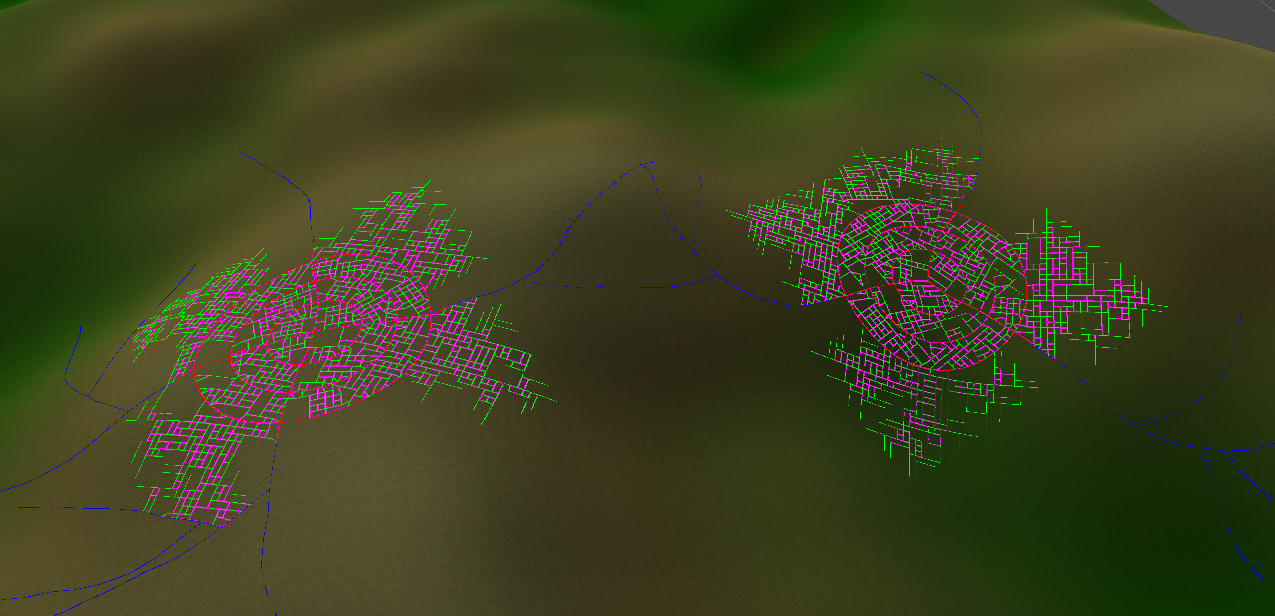
\includegraphics[width=0.8\textwidth]{figure/road_highways.png}
  \caption{Highways created outside the bounds of the city (blue lines), as well as streets (green) with blocks (purple).}

  \label{fig:road_highways}
\end{figure}

The highway strategies that were implemented into the project had a lower probability of branching than other strategies, which produced roads that were longer with fewer exits.
The aim was to produce highways that mimic the structure of highways in the real world, which this logic usually did by connecting cities together with long highways.

When the road generator is finished with the general layout of the city, the final step of generating the city roads is streets.
This was accomplished using the same road generator and Agents, but with a different strategy, which also shows the level of flexibility of the Agent-based approach.
The only difference is that these Agents start on any of the nodes in the road network and uses a street strategy, instead of starting as a city type strategy.

Furthermore, the street strategy (like other strategies) can watch the population map and react accordingly, either by changing direction or terminating the Agent.
Since the streets are a major part of the overall shape of the city, by letting the street strategy watch the population map, it could directly shape the city on a more detailed level than the city strategies could.
If the population density is too low, it could terminate the Agent, making sure it does not create streets and houses in an area where no population exists.

\subsection{Street Generation}
The street generator uses the same method as the road generator, which also shows the level of flexibility of the Agent-based approach.
The only difference is that these Agents start on any of the nodes in the road network and uses a street strategy, instead of starting as a city type strategy.

Streets are generally the same for most cities, in the sense that they are usually straight and follow a grid type of pattern.
Slight variations do exist in the real world, where some streets are curved rather than straight.
From what the group members have observed, Sweden typically has more curved streets than other countries, such as America which generally has more grid-shaped streets.
However, the basic street strategy that the method uses mimics the grid-like street style.

\subsection{City Block Generation}

A city block in this project is defined as a continuous area of land which is suitable in shape, size, and position for containing multiple buildings.
The generation of such city blocks is managed by the BlockGenerator function (see Table~\ref{table:blockgen}).

\begin{table}[H]
  \centering
  \begin{tabular}{lllll}
    \textbf{Input}                           &               & \textbf{Function}            &               & \textbf{Output}         \\
    \midrule
    \textit{RoadNetwork, PopulationMap}      & $\rightarrow$ & \textbf{BlockGenerator}      & $\rightarrow$ & \textit{Block[]}        \\
    \bottomrule
  \end{tabular}

  \caption{Definition of the BlockGenerator function which is responsible for generating city blocks.}
  \label{table:blockgen}
\end{table}
\vspace{-0.4cm} % Mimic spacing below figures

% The example labels are incorrect, but I could make a code PR that fixes that.
This function uses the road network from the road generation to find suitable areas of land to extract, and it uses the population map from the population generation to determine which type of city block it should label each area as.
Examples of such labels include: \textit{industrial}, \textit{surburbs}, \textit{downtown}, \textit{skyscrapers}, \textit{appartments} and \textit{parks.}

The labeling of city blocks was implemented in a rather simple manner.
Each label was restricted to only occur within a specific range of population density and was given a weighted probability of occurring compared to other valid labels.
In practice, this was accomplished by assigning each label a probability distribution that could then be queried using the population density of the city block area.

The trickier part was to find suitable areas of land to extract into city blocks.
One approach composed of two iterations was considered, both of which treated the road network as an undirected graph.
The first iteration would find all the minimum cycles in the road network graph and extract the area enclosed by each cycle.
These areas would then be treated as city blocks if their size and shape seemed suitable.
A limitation of this iteration was that all blocks would be perfectly enclosed by roads.

The intention of the second iteration was to supplement the first by producing new cycles instead.
The idea was to traverse the outskirts of the graph and attempt to extend imaginary nodes.
These nodes would then help form new cycles as seen in Figure~\ref{fig:extend_block}.
The imaginary nodes would solely be used for defining the areas of the new city blocks, and would not contribute to the original road network.
This iteration would help counter the limitation mentioned in the first iteration, but unfortunately, only the first iteration was implemented due to time constraints.

% Drawn using https://csacademy.com/app/graph_editor/
% Since I only show my creation (and not their site) I don't need to cite.
\begin{figure}[h!]
  \centering
  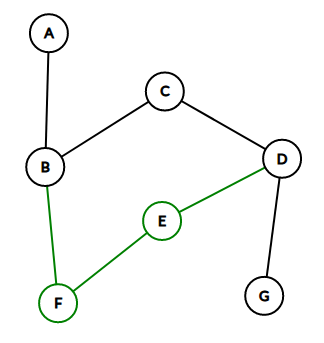
\includegraphics[width=0.35\textwidth]{figure/extend_block.png}

  \caption{Conceptual example of what the second city block extraction iteration could have produced. Here, the new cycle $BCDEF$ has been formed. Intersections are illustrated as nodes, roads as edges, and the extended block is colored green.}
  \label{fig:extend_block}
\end{figure}

The first iteration needed to find all minimum cycles in an undirected graph.
This is a known problem called Minimum Cycle Bases (MCB) and can be solved in $\mathcal{O}(m^3 + mn^2 \log n)$ or $\mathcal{O}(m^2n^2)$, for a graph with $n$ vertices and $m$ edges, using the efficient implementations proposed by Melhorn and Michail \cite{mcb_paper}.
These asymptotic time complexities might suffice for small cities, but not for multiple large ones.
Thus, either significant constraints had to be made, or another solution had to be found.

Fortunately, another solution was found.
Unlike typical graphs found in discrete mathematics, these road networks are constrained by a physical space, and are therefore a type of geometric graph.
Essentially, each node has a position relative to others and each edge has an angle relative to others.
With this information it actually becomes possible to solve the MCB problem, seemingly in only $\mathcal{O}(n + m)$.

The solution, first proposed by Petovan \cite{petovan}, can be described as follows:
\vspace{-0.5cm} % Reasonable spacing before list
\begin{enumerate}
  \item For each node, dispatch a \textit{turtle} along each connected edge.
  \item Let the \textit{turtle} traverse the graph by always following the edge closest (in counter-clockwise direction) to the previously traversed edge. Essentially, let the turtle always follow the rightmost edge relative to its current heading.
  \begin{enumerate}
    \item If the turtle tries to traverse some edge in a direction that has already been explored (potentially by another turtle), then terminate this turtle.
    \item If the turtle tries to traverse an edge it has already traversed, then terminate this turtle.
    \item If the turtle found back to the start node, then
      \begin{enumerate}
        \item if the turtle has turned an accumulated amount of 360 degrees conter-clockwise, discard it.
        \item otherwise, add the nodes the turtle visisted to a list of minimum cycles.
      \end{enumerate}
      %
  \end{enumerate}
  \item The resulting list of minimum cycles is the MCB of the graph.
\end{enumerate}

% Do we want to make a formal proof? Could be an appendix. Would be pretty cool to be first.
%The correctness nor runtime complexity of this algorithm has any known published proof, but an intution can still be gained.
Each turtle traverses the graph using the Pledge algorithm \cite{turtle_geometry}, which ensures that all non-terminated turtles will return to their start node.
The step \textit{2.a} ensures that all cycles have an area, and step \textit{2.c.i} handles the edge case where one turtle follows the perimeter of the whole graph.
The remaining cycles must be minimum since, otherwise, some edge would have to exist within the cycle but that edge would have been traversed by always following the rightmost edge, no matter the starting node (see Figure \ref{fig:graph_cycles}).
Thus, the correctness of the algorithm is shown.

% Drawn using https://csacademy.com/app/graph_editor/
\begin{figure}[h!]
  \centering
  \begin{subfigure}[b]{0.3\textwidth}
    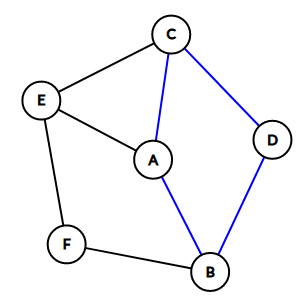
\includegraphics[width=\textwidth]{figure/blockgen1.png}
    %\caption{A minimum cycle.}
  \end{subfigure}
  \begin{subfigure}[b]{0.3\textwidth}
    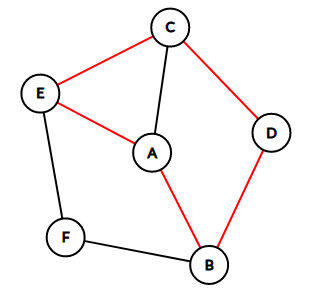
\includegraphics[width=\textwidth]{figure/blockgen2.png}
    %\caption{A non-minimum cycle.}
  \end{subfigure}

  \caption{Example of a minimum cycle (blue) and a non-minimum cycle (red). The red cycle has the edge \textit{AC} which splits the cycle into two minimum ones.}
  \label{fig:graph_cycles}
\end{figure}

Each edge is traversed twice (once from each direction) and each node is considered once for dispatching the turtles.
The rightmost edge can be queried in constant time by storing edges in counter-clockwise order in each node (and by storing array indices in the edges).
Thus, the algorithm runs in $\mathcal{O}(n + m)$.
With this efficiency, the generation of city blocks would no longer risk being a bottleneck.

Before returning, the BlockGenerator also insets the polygons of the resulting city blocks.
This step is needed to make sure the city blocks do not overlap with the road mesh of each edge.
Any further refinements of city blocks are subsequently handled by the plot generation.


\subsection{Plot Generation}  

In this project, a plot is defined as a continuous area of land within a block that is suitable for containing a single building, park, or parking lot.
The generation of such plots is managed by PlotGenerator (see Table \ref{table:plotgen}).

\begin{table}[H]
  \centering
  \begin{tabular}{lllll}
    \textbf{Input}                           &               & \textbf{Function}            &               & \textbf{Output}         \\
    \midrule
    \textit{Block, PopulationMap}            & $\rightarrow$ & \textbf{PlotGenerator}       & $\rightarrow$ & \textit{Plot[]}         \\
    \bottomrule
  \end{tabular}

  \caption{Definition of the PlotGenerator function, which is responsible to split a block into one or more plot.}
  \label{table:plotgen}
\end{table}
\vspace{-0.4cm} 

Each plot also has a label associated with it that determines what type of content should later be generated inside it. 
The label of the block, along with the population for each plot, is the deciding factor when plot labels are selected. 
For instance, if the block label is \textit{Park} or a \textit{Parking}, then the entire block is converted to one plot with the same corresponding plot label. 
However, if the block label is e.g., \textit{Downtown}, then the population density is used to sample a building from a pool of building types. 
If the population is high enough, then it is likely that the plot label will be set to \textit{Skyscraper}, to accommodate for the population. 

PlotGenerator was designed because blocks tended to be too large to suit a single structure, such as a building.
Instead of directly placing multiple buildings on a single block, the block is divided into multiple plots.
This separation of concern leads to greater modularity and makes it easier to mix a large variety of different plot labels within a single block.
The core of this plot division problem was essentially about splitting an arbitrary polygon into sensible sub-polygons. 

One of the proposed solutions was to draw a straight line through the block polygon and let the new sub-polygons be the result. 
This does not, however, result in a good split necessary. 
It is hard to control the size of the polygons, as some can become quite small. 
There is also the issue with concave polygons, where it can become difficult to create visually pleasing plots with consistency. 
There is also the issue where you can not reliably let the number of plots be a deciding factor to find the needed cut. 

% Add figures explaing.
An article about splitting polygons was found that explained how to cut a polygon into $N$ parts, where each part would have equal size \cite{polygon_splitting_article}. 
In this algorithm, each iteration finds possible cuts that could be made. 
The cuts are found by finding different ways to draw lines through what is left of the polygon. 
Some cuts are omitted in cases where concave polygons exist since they can be outside of the polygon. 
The cut that is the shortest for each sub-polygon is the one that is applied and added to the output. 
This was ultimately the algorithm used in the final product. 

\subsection{Building Generation}
The purpose of BuildingGenerator is to generate different kinds of visually pleasing buildings, everything from small houses to towering skyscrapers. 
The BuildingGenerator takes three inputs: the plot in which to build, the terrain on which to build on top of, and the population density that helps determine the size of the building \ref{table:buildinggen}.

\begin{table}[H]
  \centering
  \begin{tabular}{lllll}
    \textbf{Input}                           &               & \textbf{Function}            &               & \textbf{Output}         \\
    \midrule
    \textit{Plot, Terrain, Population}       & $\rightarrow$ & \textbf{BuildingGenerator}   & $\rightarrow$ & \textit{Building}       \\
    \bottomrule
  \end{tabular}
  
  \caption{Definition of the BlockGenerator function, which is responsible for constructing a single building on top of a plot.}
  \label{table:buildinggen} 
\end{table}
\vspace{-0.4cm} 

As buildings were considered a core part of a convincing modern city, it was essential to have a generator that could produce many different kinds of buildings. 
This problem was broken down into several sub-generators, each responsible for a particular type of building.
The plot label largely determined the sub-generator chosen for a specific plot.

% manhattan typ aktiga byggnader passar bra här
There two strategies used for generating buildings, the first of which used stochastic L-systems to generate diverse buildings.
The L-systems were implemented with type parameters to be able to handle the generation of many objects e.g. walls and floors.
The two types of parameters are the object type in the L-system and the data class that is used for the generation.
An example of the code to generate wall segments can be found in Figure \ref{fig:lsystem-example}. 
A building generated via L-systems has some generated floors, where each floor has walls and is built with multiple smaller textured wall segments. 
These wall segments include windows, shop windows, and doors.

As an example, the steps for generating a Manhattan-style skyscraper are as follows:
\begin{enumerate}
    \item An L-system is used to generate different kinds of floors for the building. These floor types indicate what kind of L-system should be used later for the generation of the wall segments. Example of floor types include:
    \begin{itemize}
        \item FirstFloor - A floor that has shop windows and doors.
        \item OnlyWindowFloor - A floor that will only have window segments. 
        \item MirrorFloor - A symmetric floor where one half of the floor segments are copied and flipped to the other half.
    \end{itemize}
    These example types are visualized in Figure \ref{fig:segmentsgen}.
    \item Each wall is then generated, floor-by-floor. Each floor type has its own L-system to generate different wall segments.
    \item The walls are then put together inside the plot, with a flat roof on top.
    \item The building is then placed on the highest point of the terrain within the plot. Basement walls are then generated downwards to connect the building with the ground. %techically it's the highest point of the plot.points
\end{enumerate}

% Explain how the direction of the wall is decide. Maybe draw a picture of it?

\begin{figure}[H]
  \centering
  \begin{subfigure}[b]{0.32\textwidth}
    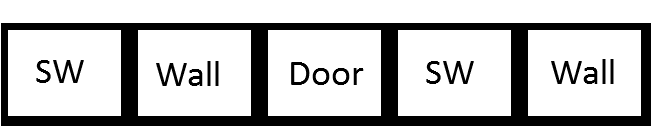
\includegraphics[width=\textwidth]{figure/FirstFloor.png}
    \caption{FirstFloor.}
  \end{subfigure}
  \quad
  \begin{subfigure}[b]{0.32\textwidth}
    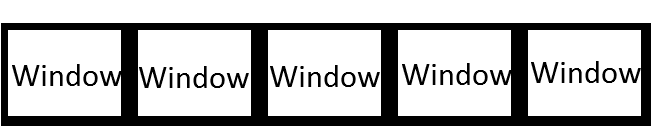
\includegraphics[width=\textwidth]{figure/OnlyWindowFloor.png}
    \caption{OnlyWindowFloor.}
  \end{subfigure}
  \begin{subfigure}[b]{0.32\textwidth}
    
\includegraphics[width=\textwidth]{figure/MirrorFloor.png}
    \caption{MirrorFloor.}
  \end{subfigure}
  \caption{Three different floor types and an example of their wall segment generation.}
  \label{fig:segmentsgen}
\end{figure}

The second strategy was only applied to certain skyscrapers and used a large texture atlas of windows from which sub-regions of windows were randomly sampled.
These skyscrapers were also adjusted in size, depending on the population.
This strategy, although quite simple, provided useful variation for windows, which tend to look a bit too similar otherwise.

%du har en stor repeating texture, två olika sådana av textures, tar små delar av den här textures, och applicerar den på olika ställen av skyskrapan
%fönstrena blir slumptade. 
%random uv koordinat
%random subbild och applicerar det i ett grid. 

\begin{figure}[H]
  \begin{lstlisting}[]
    lSystem = new LSystem<ManhattanWallSegmentType, ManhattanSegmentsGeneratorData>();

    lSystem.ShouldContinue(value => value.widthLeft > 0);

    lSystem.CreateRules(Corner)
        .Add(0.5f, Wall)
        .Add(0.5f, Window)
        .OnAccepted(value => new ManhattanSegmentsGeneratorData(value.widthLeft - cornerWidth));

    lSystem.CreateRules(Window)
        .Add(0.5f, Wall)
        .Add(0.5f, Window)
        .ShouldAccept(value => value.widthLeft >= windowWidth)
        .OnAccepted(value => new ManhattanSegmentsGeneratorData(value.widthLeft - windowWidth));

    lSystem.CreateRules(Wall)
        .Add(0.5f, Wall)
        .Add(0.5f, Window)
        .ShouldAccept(value => value.widthLeft >= wallWidth)
        .OnAccepted(value => new ManhattanSegmentsGeneratorData(value.widthLeft - wallWidth));
  \end{lstlisting}
  \label{fig:lsystem-example}
  \caption{Example of wall segment generation via L-System in code. Notice how the \textit{Wall} segment types have a 50\% chance of the next segment being another \textit{Wall}, or a \textit{Window}.}
\end{figure}

\subsection{Park Generation}
The ParkGenerator, much like the BuildingGenerator, has the primary task of filling city plots with visually pleasing, interesting content. 
To accomplish this, the ParkGenerator was implemented as a function that takes two inputs, the plot to generate the park in and the underlying terrain.
These parameters are then used to produce a park as output (see Table~\ref{table:parkgen}).

Since real-world parks come in all sizes and shapes, and can contain a variety of different objects, a scope had to be defined for what to include in the parks for this project.
For the scope of this project, the objects were limited to bushes, trees, rocks, and paths, but it was implemented in such a way that it would be simple to add more objects such as benches, fountains, and statues.

\begin{table}[H]
   \centering
   \begin{tabular}{lllll}
     \textbf{Input}                           &               & \textbf{Function}            &               & \textbf{Output}         \\
     \midrule
     \textit{Plot, Terrain}                   & $\rightarrow$ & \textbf{ParkGenerator}       & $\rightarrow$ & \textit{Park}           \\
     \bottomrule
   \end{tabular}

   \caption{Definition of the ParkGenerator function which is responsible for generating parks.}
   \label{table:parkgen}
 \end{table}
 \vspace{-0.4cm}
 
The development of the Park Generator consisted of two main phases:
\begin{easylist}
 @ Filling the park with objects such as trees, bushes, and rocks.
 @ Creating natural paths for people to walk on.
\end{easylist}
To make the parks vary in appearance through procedural generation, a way to randomize the placement of objects inside any given plot had to be constructed.
However, pure randomness of placement would produce some unrealistic results.
Another problem to tackle was the frequency of objects i.e. determining how much of each object is reasonable to have within each park. 
For example, one tree, 43 stones, and two bushes would likely look like an odd park.
 
The algorithm for generating objects was implemented by making use of uniform randomness between 0 and 10.
The range 0-10 was split into several separate, but not equally large sub-ranges, which would determine what object to generate.
For example numbers in the range [6,10] could result in a tree, [2,5] could result in a bush, and [0,1] could result in a rock.
As real-world objects are never identical, having one model for each object type would not be sufficient. 
Therefore, once the object type is decided, a model is sampled from an array of such model types, and then randomly rotated and scaled. 

It was considered important to be able to distinguish the park-objects based on size and type as these parameters would determine how far from each other objects would be allowed to be generated.
This is referred to as giving each object-type a radius relative to other object-types.
A function was then constructed to search within the radius of each object and make sure no object could be created within another object's radius (see Figure~\ref{fig:radius}).
This implementation is based on Poisson Disc Sampling \cite{poisson_fast} in a manner that it scatters points randomly across the plot, while maintaining a distance from each already created point.
Here the object-radius is used in order to determine how closely objects may stack. 
When the paths were implemented, a slight adjustment also had to be made to the algorithm for object placement, such that all objects took into consideration the coordinates of the path and were not placed on top of it.
\begin{figure}[H]
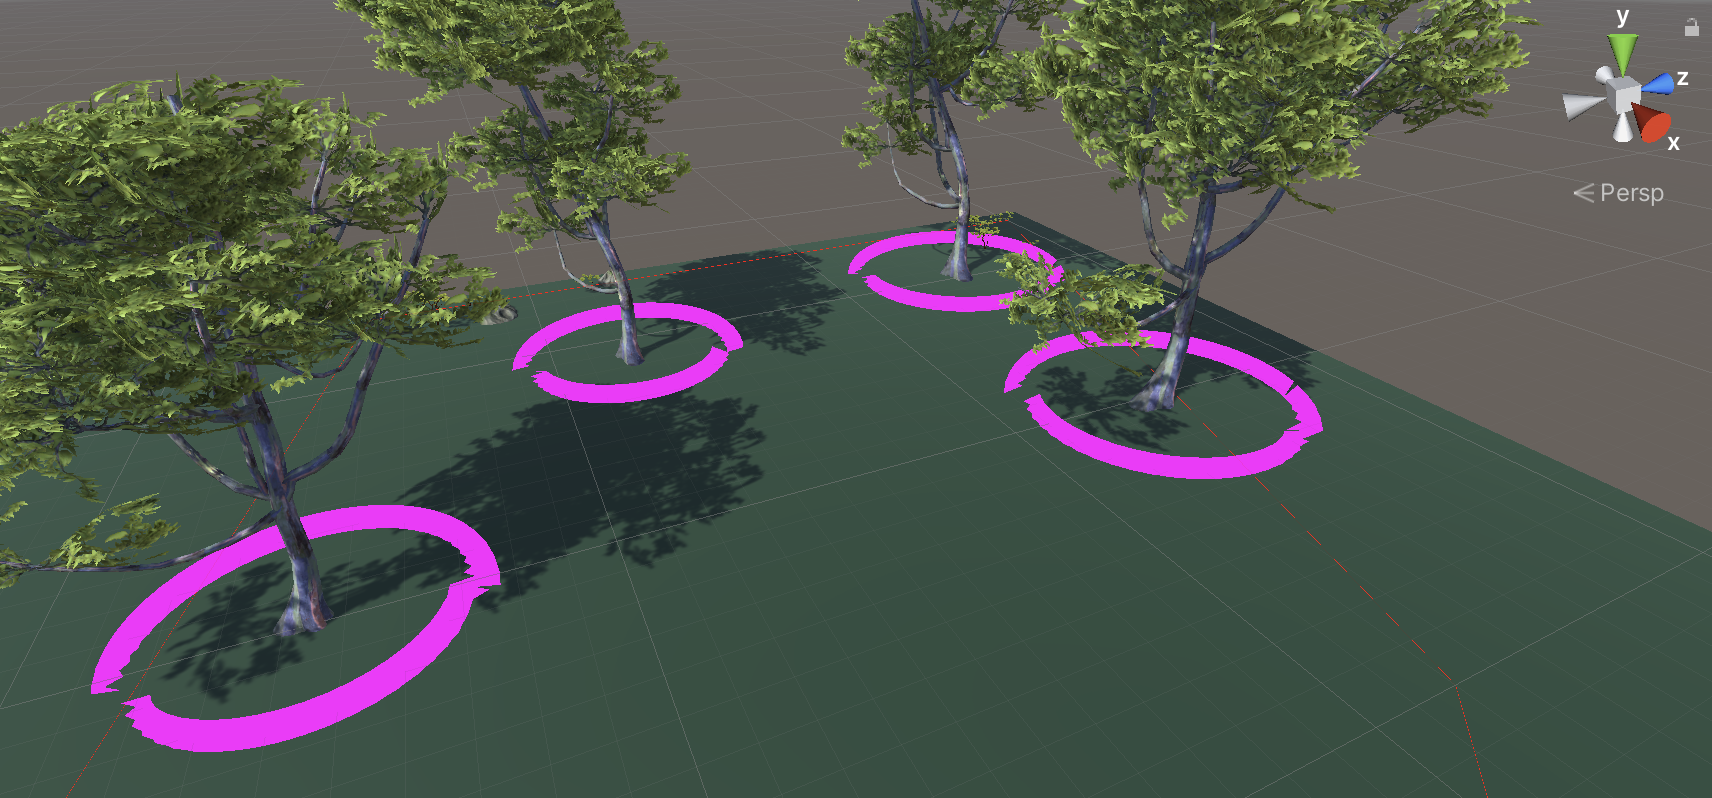
\includegraphics[width=\linewidth]{figure/radiuscontrol.png}
\caption{Radius of the tree object shown in pink. This radius indicates how closely trees may pack.}
\label{fig:radius}
\end{figure}

The algorithm for creating paths was inspired by Cyclic Dungeon Generation \cite{cyclic}.
The main takeaway from that concept was that a start and goal node was generated for the algorithm to create a loop between.
Having a loop would allow for people to take a stroll around the park and return to where they entered, and based on observation, this is also a frequently occurring pattern for paths in real-world parks. 

The development of the path generation can be described as three iterations of implementation.
The first implementation of the algorithm created two random points within the plot, one as start and another one as goal. 
The program then traveled the park at random until it found a path to the goal, at which point it would find a new way back to the starting point. 
It was however, quickly discovered that this approach had some problems.
 
One of these problems were that the paths would look unnatural when taking steps far away from the goal. 
A solution to this was to revert the path to its previous node if it took a step which was further away from the goal than it had previously been, this was an instant improvement in appearance. 
However, after observing many of the generated paths from this approach the paths still looked linear. 
This was believed to be because simply going from one point to another and not straying off too much from the goal could not produce much more interesting results than that (see Figure~\ref{fig:linear}).
\begin{figure}[H]
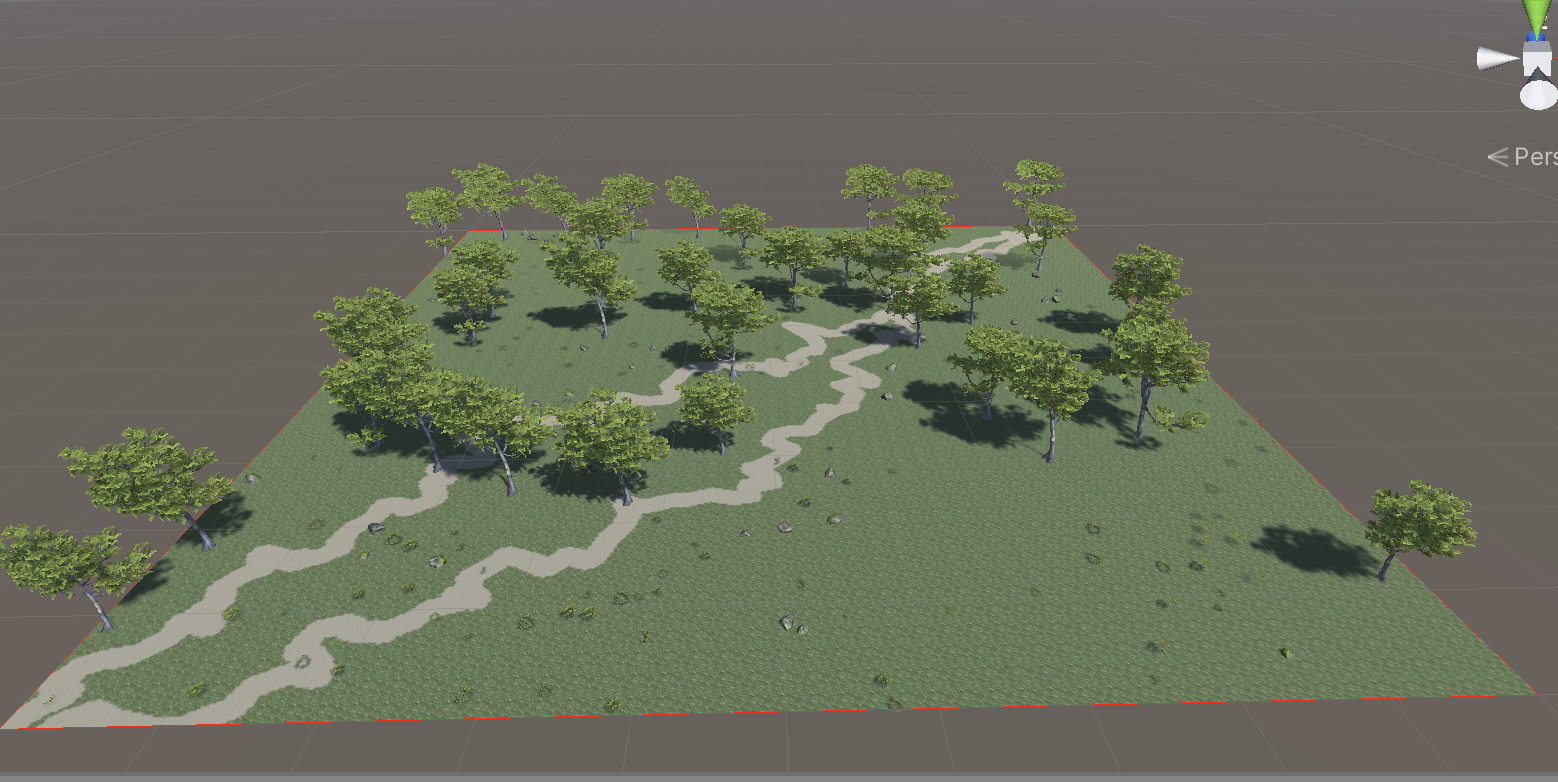
\includegraphics[width=\linewidth]{figure/linear.png}
\caption{Example of a path generated by the first implementation of the algorithm.}
\label{fig:linear}
\end{figure}
The second implementation of the algorithm was inspired by the flaws which had been demonstrated by its predecessor, more specifically its linear shapes and its tendency to create steps with abrupt angle-changes.
As a result of this, it was for the second implementation decided that rather than having a start and goal, the path would consist of an array of points, which all had to be visited before the path would be completed.
This was changed in order to try to get rid off the linearity presented in the first implementation.
For this implementation a control of how many degrees a step in the path could differ from the current point to its previous step was also added.
This was done to avoid the zigzag-like patterns caused by the angle-changes from the first implementation.
The second implementation would just like the first one look for one assigned point, but in this case start searching for the next point after finding the previous one and continue doing so until all points have been found (see Figure~\ref{fig:texsplat}). 
\begin{figure}[H]
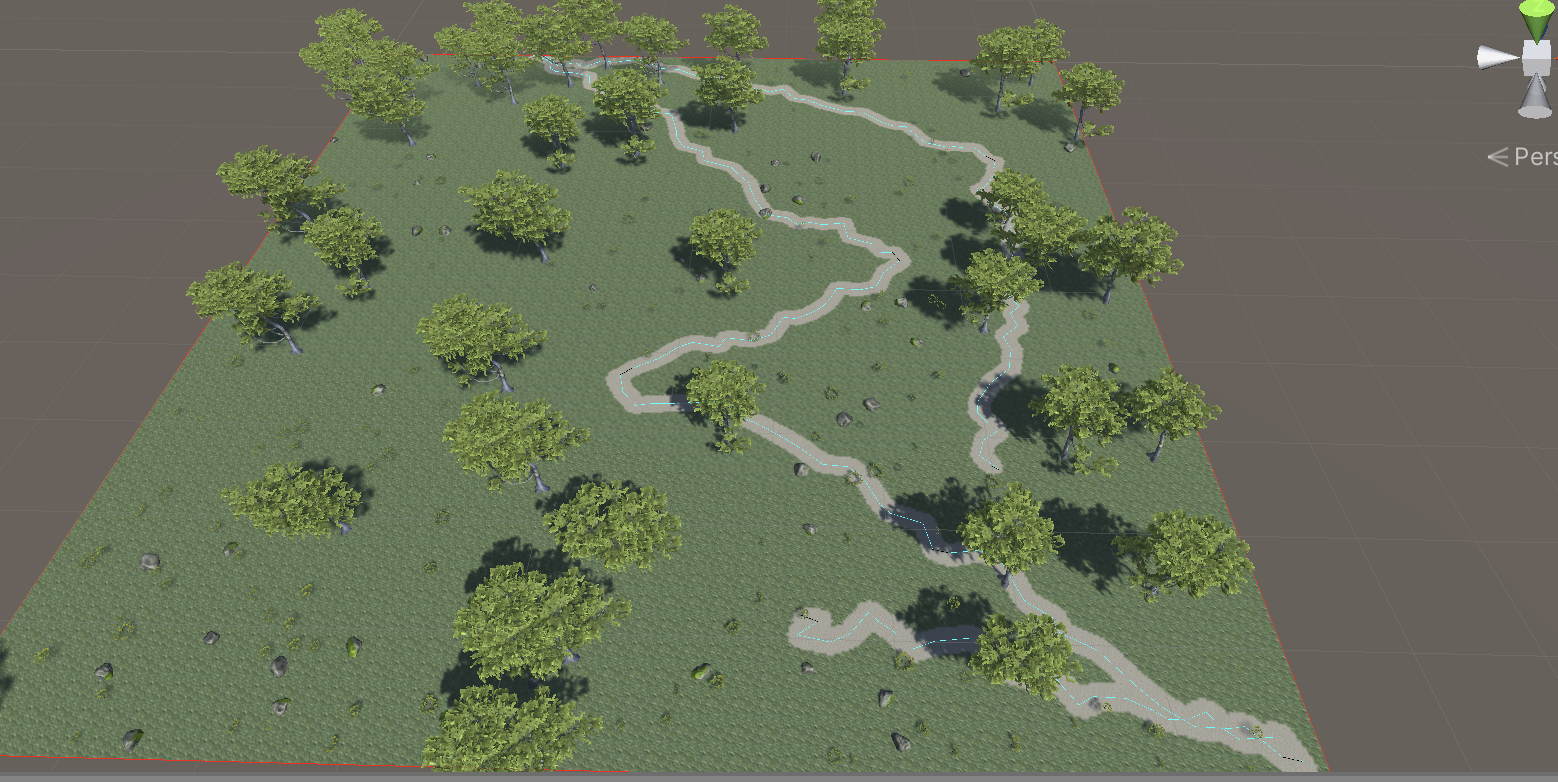
\includegraphics[width=\linewidth]{figure/texturesplat}
\caption{Example of a path generated by the second implementation of the algorithm.}
\label{fig:texsplat}
\end{figure}
The third and final implementation made use of a similar algorithm.
Some fairly small changes were made in order to address the issues experienced with the second implementation.
The second implementation would still create paths starting in the middle of the park which did not make a lot of sense, this was handled by always creating the start node on one of the edges of the plot.
The algorithm then creates an additional number of randomly placed points, based on the size of the plot.
Having this number be based on the size of the plot made for some more interesting and realistic results which was lacking in the second implementation.

Afterwards, the points are sorted by distance to enforce that the algorithm always traverses towards the point closest to itself. 
This change was inspired by seeing some paths traverse towards points far away from the starting point only to then traverse to a point close to the starting point.
Once all goal points have been reached a path is either created back to the starting node, or a new path is created to a randomly selected edge on the plot. 
This change was made to stop enforcing loops and to add more variety to the generated paths.
Finally, the algorithm creates exits/entries to the park by projecting a line to closest edge of the plot from some of the points, and then creating a path between them. 
 
The visual implementation of the paths was done by texture splatting on top of a Unity Terrain for the first two implementations (see Figure~\ref{fig:linear} and Figure~\ref{fig:texsplat}).
However, as the Unity Terrain needed to be replaced with a mesh generated one, this had to be re-implemented for the third implementation.
Some different approaches for visualizing the paths were investigated, such as using quad and sphere meshes and then simply placing these along each path.
The spheres would cause a shape that was still distinguishably circular and the quads would likewise create patterns that were clearly square. 
The final implementation would instead make use of the logic from the RoadGenerator to create its own internal road network, thereby inheriting the functionality used to generate the corresponding mesh (see Figure~\ref{fig:visuals}).
\begin{figure}[H]
  \centering
  \begin{subfigure}[b]{0.4\textwidth}
    \frame{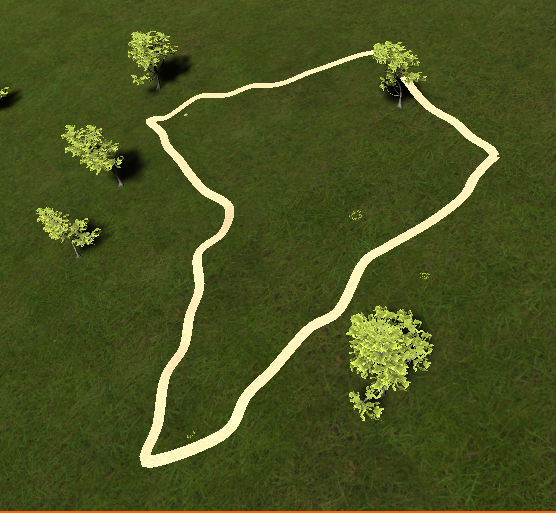
\includegraphics[width=\textwidth]{figure/splinepath}}
    \caption{Visualization of a path using splines.}
  \end{subfigure}
  \quad
  \begin{subfigure}[b]{0.3\textwidth}
    \frame{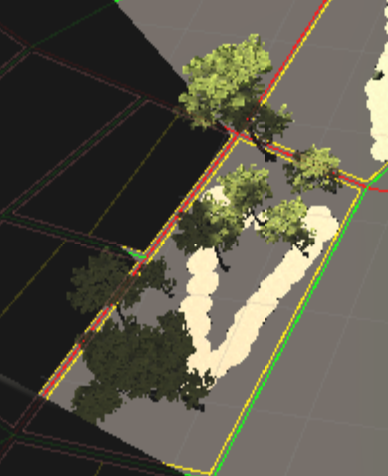
\includegraphics[width=\textwidth]{figure/spherepath}}
    \caption{Visualization of a path using spheres.}
  \end{subfigure}
  \caption{Two of the approaches for visualizing paths on top of the mesh generated terrain.}
  \label{fig:visuals}
\end{figure}

\subsection{Parking Lot Generation}
The ParkingGenerator is implemented as a function that takes a plot and its underlying terrain as input and produces a parking lot as output (see Table~\ref{table:parking}).
This generator in particular is responsible for filling roughly ten percent of the generated cities with parking lots, a percentage based on research conducted in Phoenix,~AZ~\cite{parking_percent}.
\begin{table}[H]
   \centering
   \begin{tabular}{lllll}
     \textbf{Input}                           &               & \textbf{Function}            &               & \textbf{Output}         \\
     \midrule
     \textit{Plot, Terrain}                   & $\rightarrow$ & \textbf{ParkingGenerator}       & $\rightarrow$ & \textit{Parking lot}           \\
     \bottomrule
   \end{tabular}

   \caption{Definition of the ParkingGenerator function which is responsible for generating parking lots.}
   \label{table:parking}
 \end{table}
 \vspace{-0.4cm}

One considered approach for generating parking lots was Esri CityEngine's \cite{Esri}.  % having a hard time finding this source, Anton who found it... plz help me. 
What they use, for at least some of their generation is simply covering areas with textures. This can be seen in their parks and parking lots. 
This was at first considered to be a viable option for the project, only it was found that it offers little alternatives for modification.

Modification, in this remark, includes the shape of the entire parking lot as well as the size of the individual parking spaces.
As every other generator provides fully scalable content, it would be inconvenient for the ParkingGenerator to be any different.
By using a single mesh with one texture applied to it, it would remove the possibility of scaling the size of the parking spaces within the mesh without scaling the mesh itself, which is not an option.

Another approach that was considered, was to generate each line in the parking area individually. 
This was the initial approach that was used in the application, but due to performance concerns when dealing with multiple line objects, this had to be changed.

The final approach was a combination of the Esri method, and the method which had been previously used. 
The first step of this approach is to fill the plot with asphalt, but this is not an easy task as the mesh that is projected has to be perfectly aligned with the terrain mesh.
In order to avoid clipping issues, the algorithm basically cuts out a portion of the terrain in the shape of the plot, and then slightly offsets it upwards.
As a result of this, the mesh will never clip with the terrain. 

Afterward, a function for approximating the largest rectangle inside a polygon is applied to the plot to find a suitable rectangle to generate parking lots in.
Based on the size of the approximated rectangle, the algorithm generates as many rows of parking lots as it can fit.
Each row contains a quad that is projected onto the terrain with a transparent texture with only the white parking lot lines in it.
By modifying the UV coordinates of the quad, the texture can be repeated and scaled to the right size.
The plot is also given a certain margin around it to make sure there is enough space around the parking lots for cars to get in and out of the parking area.

The reasoning behind this algorithm was the group's observation that parking lots seem to have a rectangular shape generally (see Figure~\ref{fig:parkings}).
This shape does of course not apply to every parking lot in the world, however attempting to create parking lots of any size and shape would require a lot more effort, and was therefore deemed out of scope for this project. 

\begin{figure}[H]
  \centering
  \begin{subfigure}[b]{0.55\textwidth}
    \frame{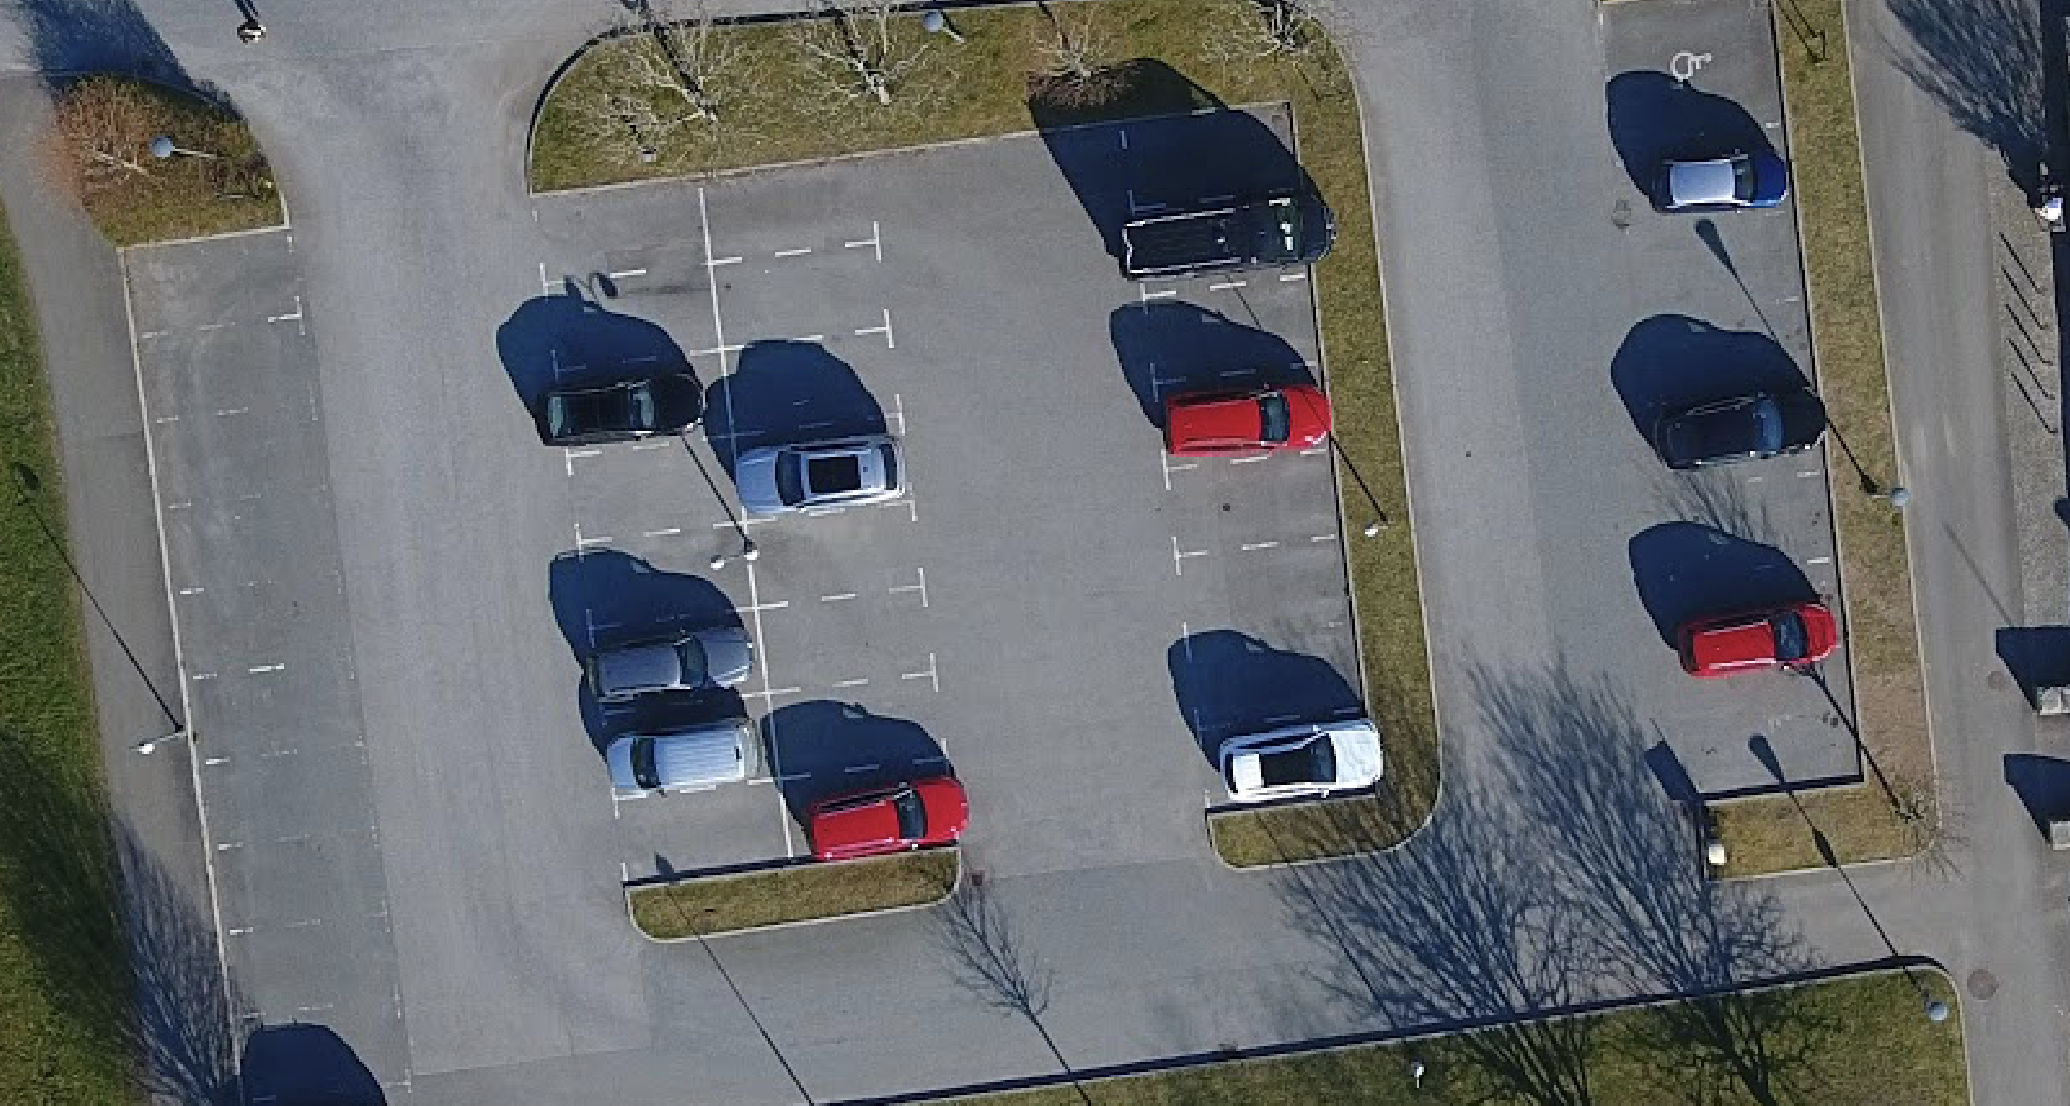
\includegraphics[width=\textwidth]{figure/parking1}}
  \end{subfigure}
  \quad
  \begin{subfigure}[b]{0.395\textwidth}
    \frame{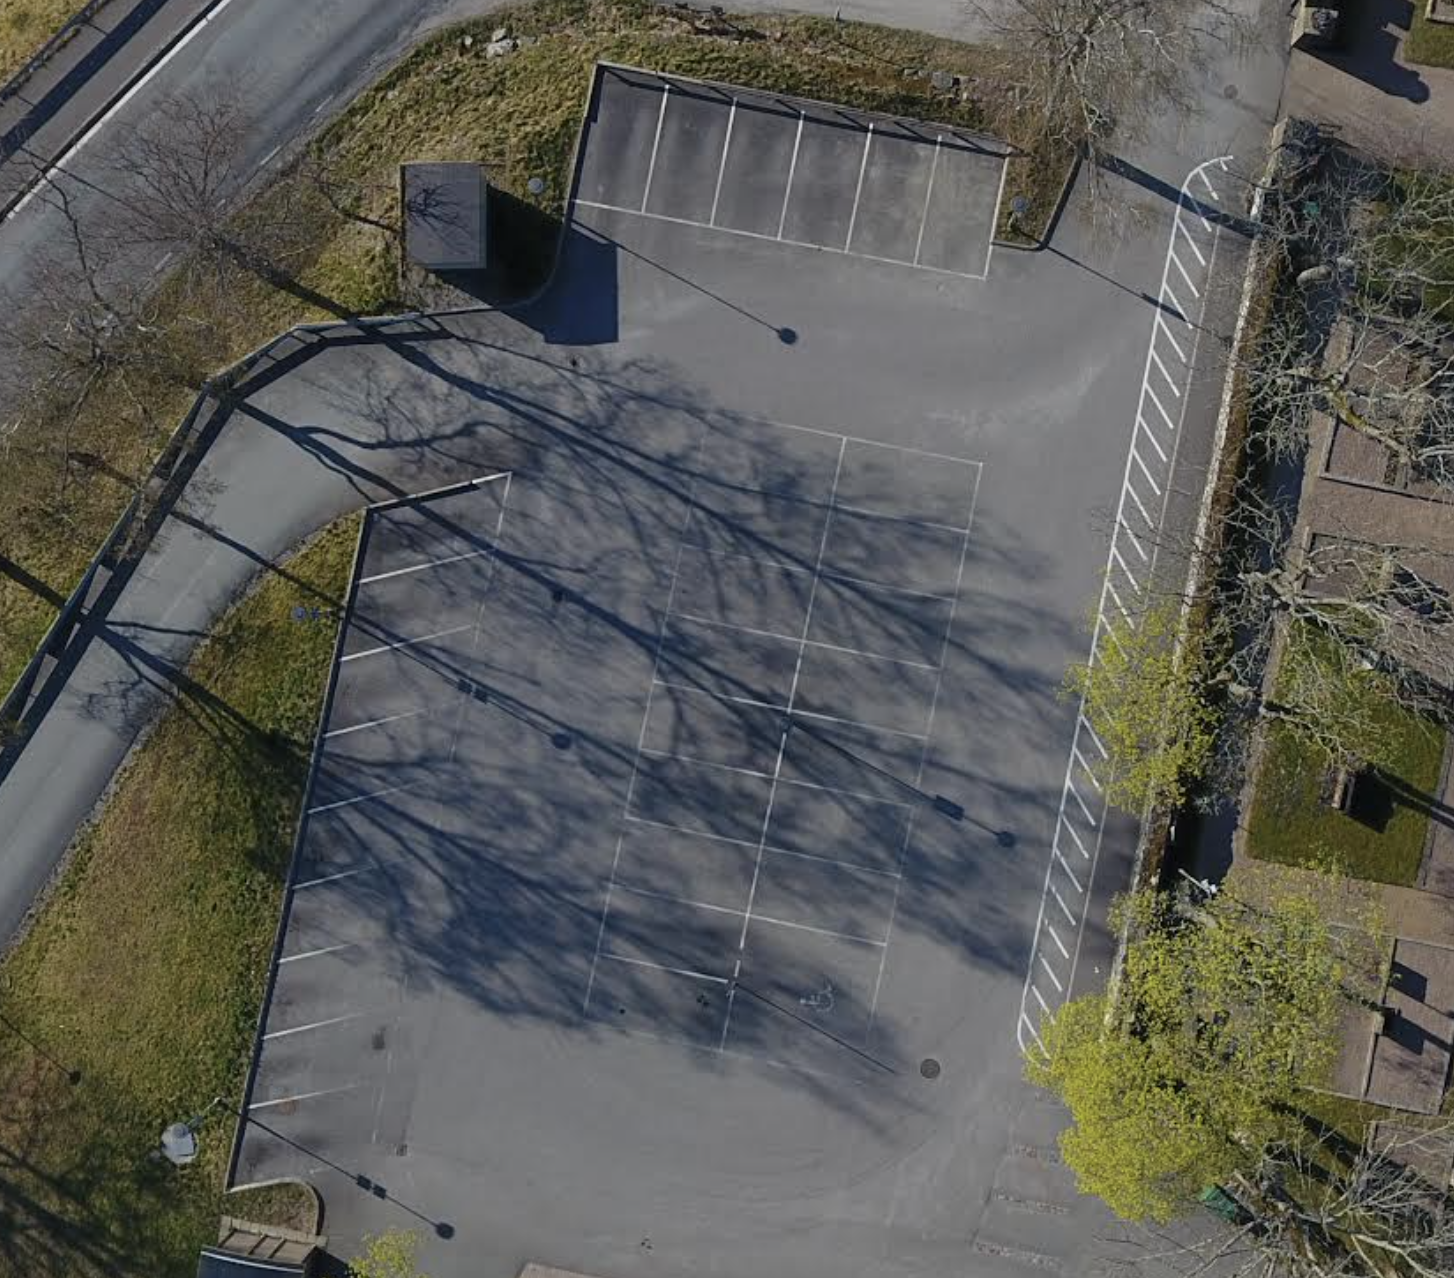
\includegraphics[width=\textwidth]{figure/parking2}}
  \end{subfigure}
  \caption{Two examples of parking lots observed by the project group, showcasing the rectangular shapes mentioned above.}
  \label{fig:parkings}
\end{figure}

\begin{figure}[H]
  \centering
  \begin{subfigure}[b]{0.485\textwidth}
    \frame{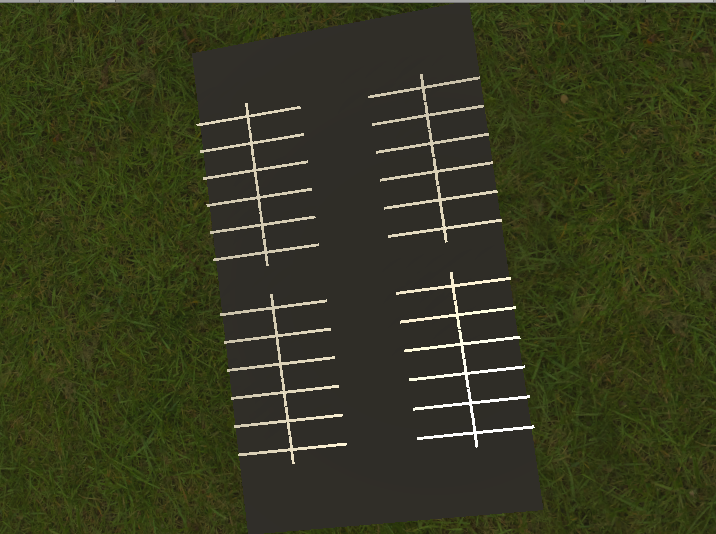
\includegraphics[width=\textwidth]{figure/fourcol}}
    \caption{Large parking lot consisting of four columns.}
  \end{subfigure}
  \quad
  \begin{subfigure}[b]{0.45\textwidth}
    \frame{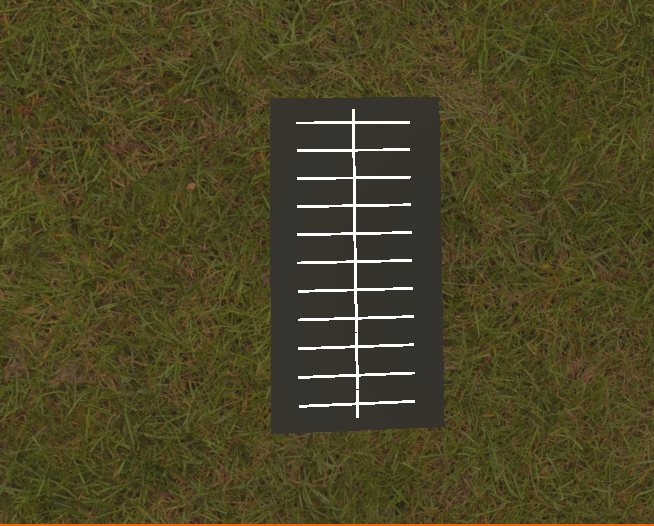
\includegraphics[width=\textwidth]{figure/twocol}}
    \caption{Small parking lot consisting of two columns.}
  \end{subfigure}
    \caption{Two examples of different sized parking lots created by the generator.}
  \label{fig:sizebased}
\end{figure}
